\documentclass[a4paper, 11pt]{article}
\usepackage{graphicx}
\usepackage{amsmath}
\usepackage[pdftex]{hyperref}
\usepackage{algorithm}
\usepackage{algorithmic}
\usepackage{epstopdf}

% Lengths and indenting
\setlength{\textwidth}{16.5cm}
\setlength{\marginparwidth}{1.5cm}
\setlength{\parindent}{0cm}
\setlength{\parskip}{0.15cm}
\setlength{\textheight}{22cm}
\setlength{\oddsidemargin}{0cm}
\setlength{\evensidemargin}{\oddsidemargin}
\setlength{\topmargin}{0cm}
\setlength{\headheight}{0cm}
\setlength{\headsep}{0cm}

\renewcommand{\familydefault}{\sfdefault}

\title{Data Mining: Learning from Large Data Sets - Spring Semester 2014 Project 1}
\author{nivo@student.ethz.ch\\ ganzm@student.ethz.ch\\ rohrp@student.ethz.ch\\}
\date{\today}

\begin{document}
\maketitle

\section*{Approximate near-duplicate search using Locality Sensitive
Hashing} 

This document explains the implementation of project 1. In this first project we
were supposed to find near-duplicate videos using Locality Sensitive Hashing.
The videos were given as a number of shingles that could be compared. The
implementation was done in Python to be used in combination with the hadoop
infrastructure. This means we implemented a mapper and a reducer that read from
stdin and write to stdout. In the following two sections we explain the
functionality of the mapper and the reducer each.

\subsection*{mapper.py}

The mapper creates a signature vector of a video. This signature
vector is afterwards subdivided into $b$ bands having $r$ elements that get
hashed. Each band and its hash are then emitted.

These are the steps in more detail:

\begin{enumerate} 

\item As \autoref{fig:func} shows, choosing $b=32$ and $r=8$ does not miss any true positives.

\begin{figure}
\centering
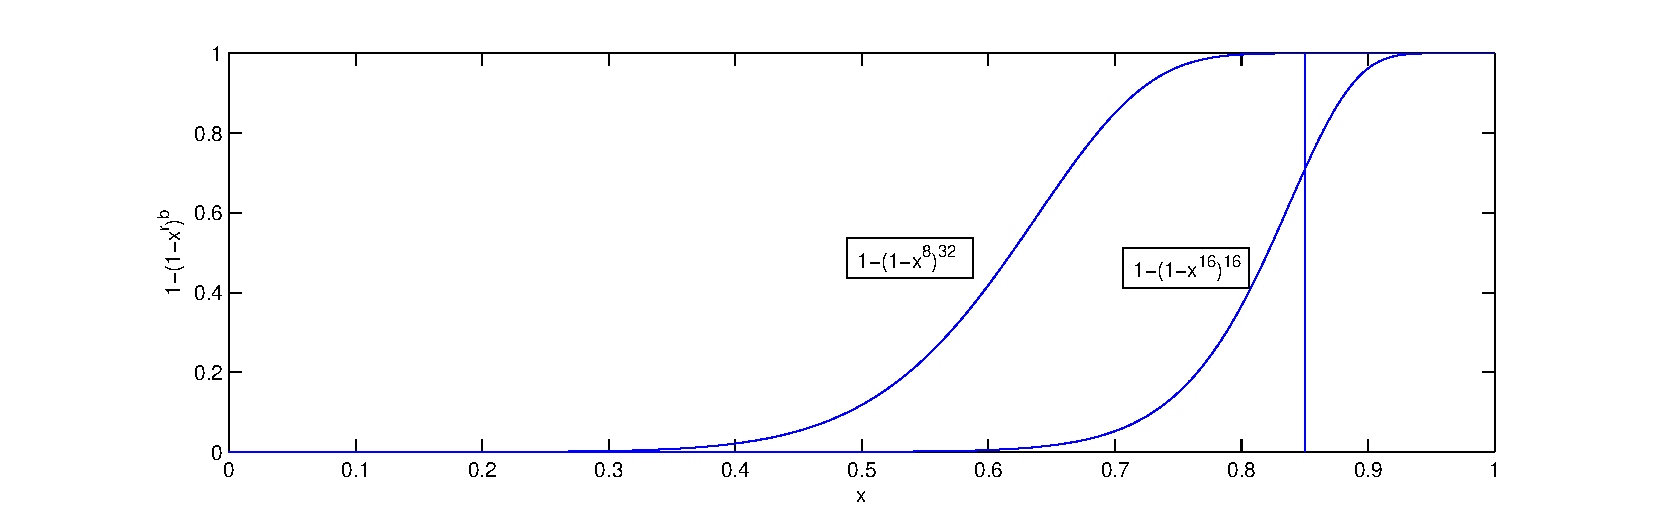
\includegraphics[scale=.7]{func.eps}
\caption{$1-(1-x^r)^b$}\label{fig:func}
\end{figure}

\item We create $k = b \cdot r$ hashfunctions of the form $ a_px + b_p \mod c_p$
where $a_p=rand(0,999), b_p=rand(0,99999)$, $c_p=10000$ and $rand(x,y)$ is
random variable drawn from a uniform distribution between $x$ and $y$. These
hashfunctions are used to calculate the permutations used for min-hashing.

\item We create $r$ hashfunctions of the form $ a_bx + b_b \mod c_b$ where
$a_b=rand(0,999), b_b=rand(0,999)$, $c_b=1000$ and $rand(x,y)$ is random
variable drawn from a uniform distribution between $x$ and $y$. These
hashfunctions are used to calculate the band hashes before emitting.

\item The signature is then created according to \autoref{alg:signature}

\begin{algorithm}

\caption{Create signature}\label{alg:signature}

\begin{algorithmic} 

\STATE $signature = \infty$

\FORALL{shingle in shingles}

\FOR{i in range(k)}

\STATE{ $signature[i] =min ({a_p}_i \cdot shingle + {b_p}_i \mod c_p,
signature[i])$}

\ENDFOR

\ENDFOR

\end{algorithmic} \end{algorithm}


\item Calculate the band hash and emit the band hash and the band as key, and
the video with its corresponding shingles as value according to
\autoref{alg:emit}

\begin{algorithm}
\caption{Emit keys and values}\label{alg:emit}
\begin{algorithmic} 

\FOR{band in range(b)}

\STATE{ $vector = signature[band \cdot r : band \cdot r + r]$}

\STATE{ $band hash = \sum_{i=1}^{len(vector)}{ {a_b}_i\cdot vector[i] + {b_b}_i \mod c}$}

\STATE{ emit $key=[band hash, band]$ $value=[video\_id, shingles]$ }

\ENDFOR

\end{algorithmic} \end{algorithm}


\end{enumerate}


\subsection*{reducer.py}

The main task of the reducer is to get rid of the false positives by comparing
the reported similar videos using the jaccard distance:

\begin{enumerate}

\item gather all videos with the same key in a collection $duplicates$
\item emit similar videos like shown in \autoref{alg:reducer}

\begin{algorithm}
\caption{Emit similar videos}\label{alg:reducer}
\begin{algorithmic} 

\FOR{i=0 to len(duplicates)}

\FOR{j=i+1 to len(duplicates)}

\IF{$duplicates[i].video\_id < duplicates[j].video\_id$}

\STATE{ $shingles\_left = duplicates[i].shingles$}
\STATE{ $shingles\_right = duplicates[j].shingles$}

\STATE{ $distance = \frac{\left| shingles\_left \cap shingles\_right \right|}{\left| shingles\_left \cup shingles\_right \right|}$}

\IF{$distance > 0.85$}

\STATE{ emit duplicates[i].video\_id duplicates[j].video\_id }

\ENDIF

\ENDIF

\ENDFOR

\ENDFOR

\end{algorithmic} \end{algorithm}


\end{enumerate}


\end{document} 
